% ------------------------------------------------
% ARQUIVO DE TESTE — variações do tema minimalista amarelo
% Cada variação mostra: capa, slide de conteúdo com tabela e slide com gráfico.
% ------------------------------------------------
\documentclass{beamer}

\usepackage{xcolor}
\usepackage[utf8]{inputenc}
\usepackage[T1]{fontenc}
\usepackage{lmodern}
\usepackage[brazil]{babel}
\usepackage{graphicx}
\usepackage{booktabs}

\definecolor{myyellow}{RGB}{220,170,0}
\definecolor{myyellowvivo}{RGB}{255,200,40}
\definecolor{grafite}{RGB}{26,26,26}
\definecolor{textoclaro}{RGB}{230,230,230}
\definecolor{cinzaescuro}{RGB}{60,60,60}

\setbeamertemplate{navigation symbols}{}

\title{Classificação Automática de Modulações}
\subtitle{Aplicações em Internet das Coisas}
\author{João Marco Pereira \\ Ricardo Alexandre Vieira da Silva}
\institute{CEFET/RJ}
\date{2026}

% Slide separador entre variações
\newcommand{\separador}[2]{%
\begin{frame}[plain]
  \vfill
  \centering
  {\usebeamercolor[fg]{frametitle}\Huge\bfseries #1}\\[4mm]
  {\large #2}
  \vfill
\end{frame}}

% Conteúdo de exemplo (igual em todas as variações, para comparação justa)
\newcommand{\slideconteudo}{%
\begin{frame}{Exemplo de conteúdo}
  Frase de texto corrido para avaliar o contraste do corpo do slide.
  \medskip
  \begin{itemize}
    \item Item com \textbf{negrito} e \texttt{2L\_64-128} em monoespaçada
    \item Item com ênfase em \emph{itálico}
    \item Terceiro item para ver o marcador
  \end{itemize}
  \medskip
  \centering
  \small
  \begin{tabular}{llrr}
    \toprule
    Grupo & Arquitetura & Média (\%) & Máx (\%) \\
    \midrule
    AM  & \texttt{2L\_64-128} & 77,99 & 79,40 \\
    AM  & \texttt{2L\_32-64}  & 77,51 & 78,64 \\
    QAM & \texttt{2L\_32-64}  & 20,00 & 20,00 \\
    \bottomrule
  \end{tabular}
\end{frame}}

\newcommand{\slidegrafico}{%
\begin{frame}{Exemplo com gráfico}
  \centering
  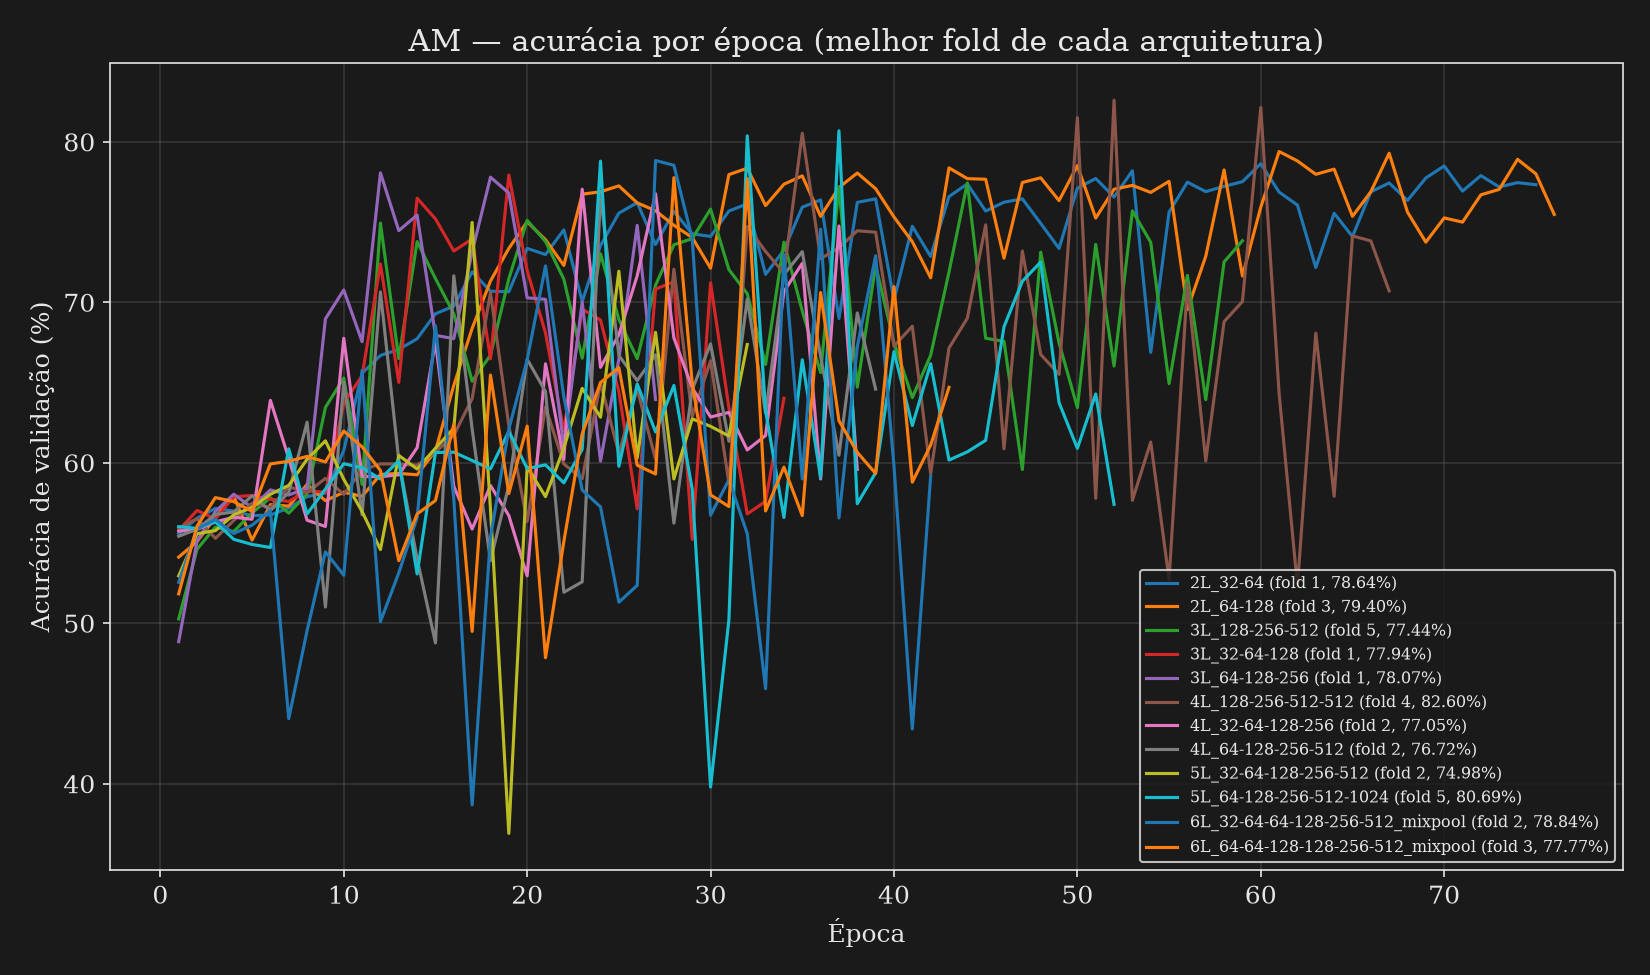
\includegraphics[height=0.75\textheight]{kfold_analysis/AM_epochs_best_fold.png}
\end{frame}}

\begin{document}

% ════════════════════════════════════════════════
% VARIAÇÃO 1 — fiel ao template original
% ════════════════════════════════════════════════
\setbeamercolor{title}{fg=myyellow}
\setbeamercolor{frametitle}{fg=myyellow}
\setbeamercolor{structure}{fg=myyellow}

\separador{Variação 1}{Fiel ao template original: amarelo puro sobre fundo branco}

\begin{frame}
  \titlepage
\end{frame}
\slideconteudo
\slidegrafico

% ════════════════════════════════════════════════
% VARIAÇÃO 2 — amarelo com régua e numeração
% ════════════════════════════════════════════════
\setbeamertemplate{frametitle}{%
  \vspace{2.5mm}%
  {\usebeamerfont{frametitle}\usebeamercolor[fg]{frametitle}\bfseries\insertframetitle}\par
  \vspace{1.2mm}{\color{myyellow}\hrule height 1.2pt}\vspace{2mm}}
\setbeamertemplate{footline}{%
  \hfill{\color{gray}\scriptsize\insertframenumber}\hspace{3mm}\vspace{2mm}}

\separador{Variação 2}{Título em negrito com régua amarela e numeração de página}

\begin{frame}
  \titlepage
\end{frame}
\slideconteudo
\slidegrafico

% ════════════════════════════════════════════════
% VARIAÇÃO 3 — barra amarela no título
% ════════════════════════════════════════════════
\setbeamertemplate{footline}{}
\setbeamercolor{frametitle}{fg=black,bg=myyellow}
\setbeamertemplate{frametitle}{%
  \nointerlineskip
  \begin{beamercolorbox}[wd=\paperwidth,sep=2.5mm]{frametitle}
    \usebeamerfont{frametitle}\bfseries\insertframetitle
  \end{beamercolorbox}}

\separador{Variação 3}{Título em barra amarela cheia com texto preto}

\begin{frame}
  \titlepage
\end{frame}
\slideconteudo
\slidegrafico

% ════════════════════════════════════════════════
% VARIAÇÃO 4 — modo escuro
% ════════════════════════════════════════════════
\setbeamertemplate{frametitle}[default]
\setbeamercolor{background canvas}{bg=grafite}
\setbeamercolor{normal text}{fg=textoclaro}
\setbeamercolor{title}{fg=myyellowvivo}
\setbeamercolor{frametitle}{fg=myyellowvivo,bg=grafite}
\setbeamercolor{structure}{fg=myyellowvivo}
\usebeamercolor[fg]{normal text}

\separador{Variação 4}{Modo escuro: fundo grafite com amarelo mais vivo}

\begin{frame}
  \titlepage
\end{frame}
\slideconteudo
\slidegrafico

% ════════════════════════════════════════════════
% VARIAÇÃO 4B — modo escuro com gráficos em fundo grafite
% ════════════════════════════════════════════════
\separador{Variação 4B}{Mesmo modo escuro, mas com os gráficos regenerados em fundo grafite}

\begin{frame}{Exemplo com gráfico (fundo grafite)}
  \centering
  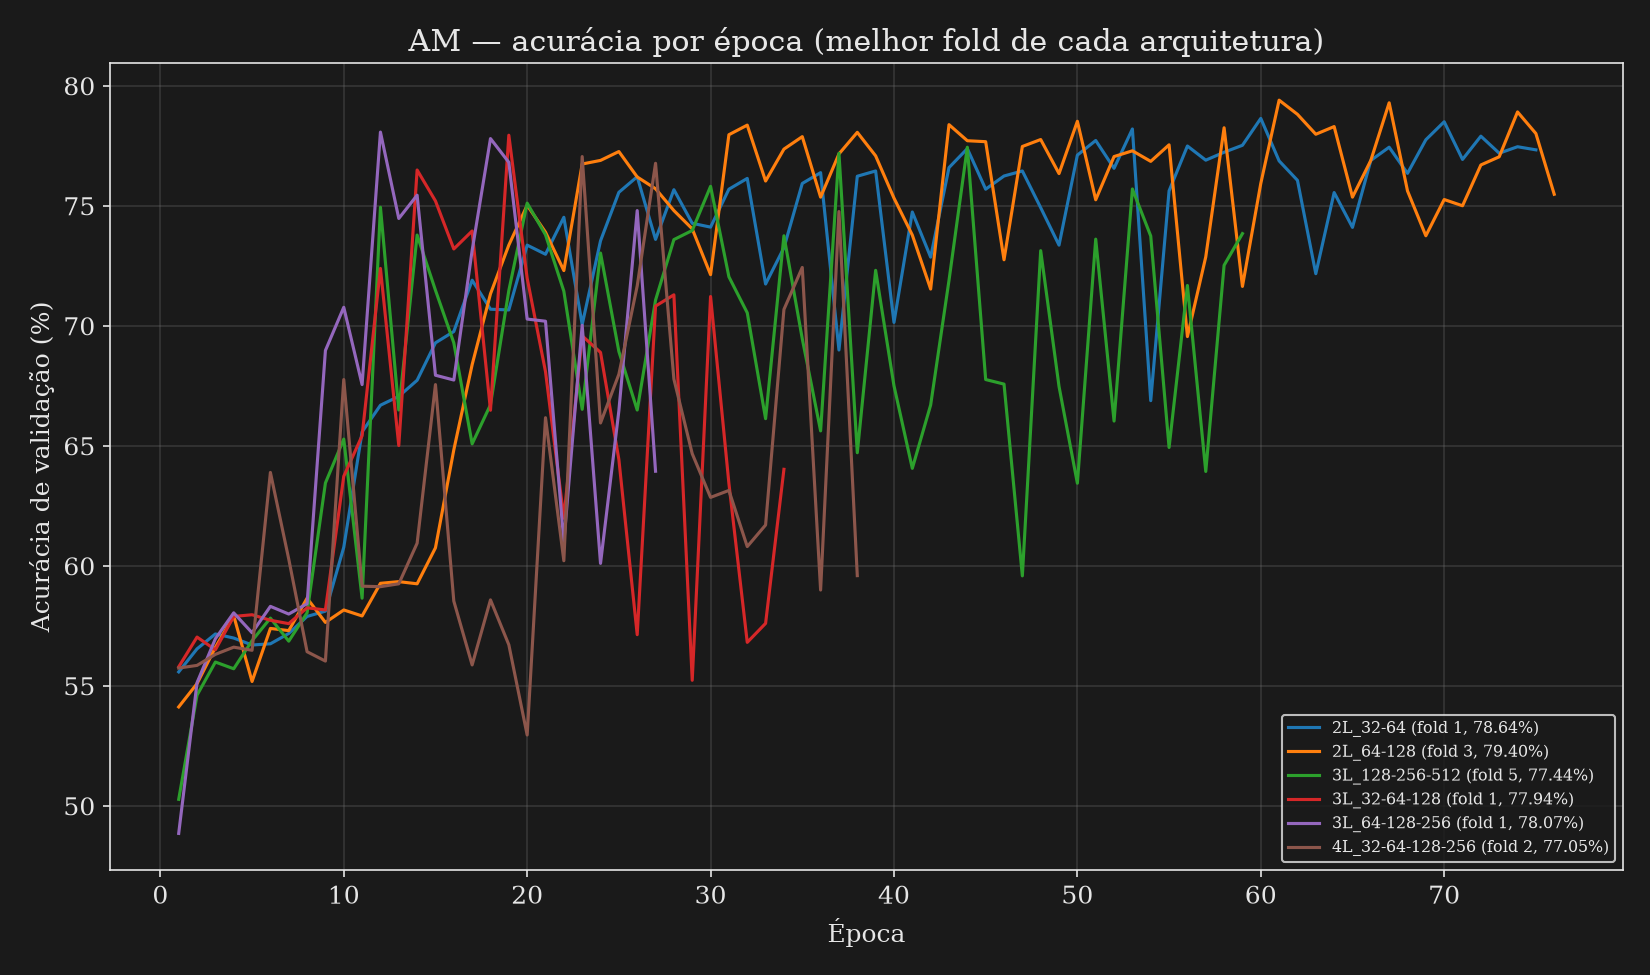
\includegraphics[height=0.75\textheight]{kfold_analysis/AM_epochs_best_fold_dark.png}
\end{frame}

\end{document}
